\documentclass[11pt,a4paper]{article}

\usepackage[utf8x]{inputenc}   % omogoča uporabo slovenskih črk kodiranih v formatu UTF-8
\usepackage[slovene]{babel}    % naloži, med drugim, slovenske delilne vzorce

\usepackage[hyphens]{url}
\usepackage{hyperref}

\usepackage{graphicx}

\title{Naslov predvidene diplomske naloge\\
\textsc{dispozicija}}
\author{Ime Priimek\\
e-naslov\\
\ \\
predvideni MENTOR: (viš. pred./doc./prof.) dr. X Y \\
Fakulteta za računalništvo in informatiko Univerze v Ljubljani
\date{\today}         
}



\begin{document}
\maketitle

\begin{abstract}
Napiši povzetek v največ 250 besedah.
\end{abstract}


\section{Motivacija za izbrano diplomsko temo}

Kaj je izhodišče za predlagano diplomsko temo? 
Ali rešuje kakšen konkreten problem? 
Ali demonstrira uporabo neke določene metode ali tehnologije?
Ali izboljšuje dosedanji način dela na nekem področju?
Komu bodo rezultati koristili?

\subsection{Pregled področja in sorodnih del}

Kaj je ``state of the art'' na področju diplomske naloge?
Izberi nekaj najbolj sorodnih del in jih na kratko opiši!


\subsection{Zakaj je predlagani mentor primeren}

Po kakšnih kriterijih si ga izbral?



\section{Miselni diagram za izbrano temo diplomske naloge}

\begin{figure}[p]
\centerline{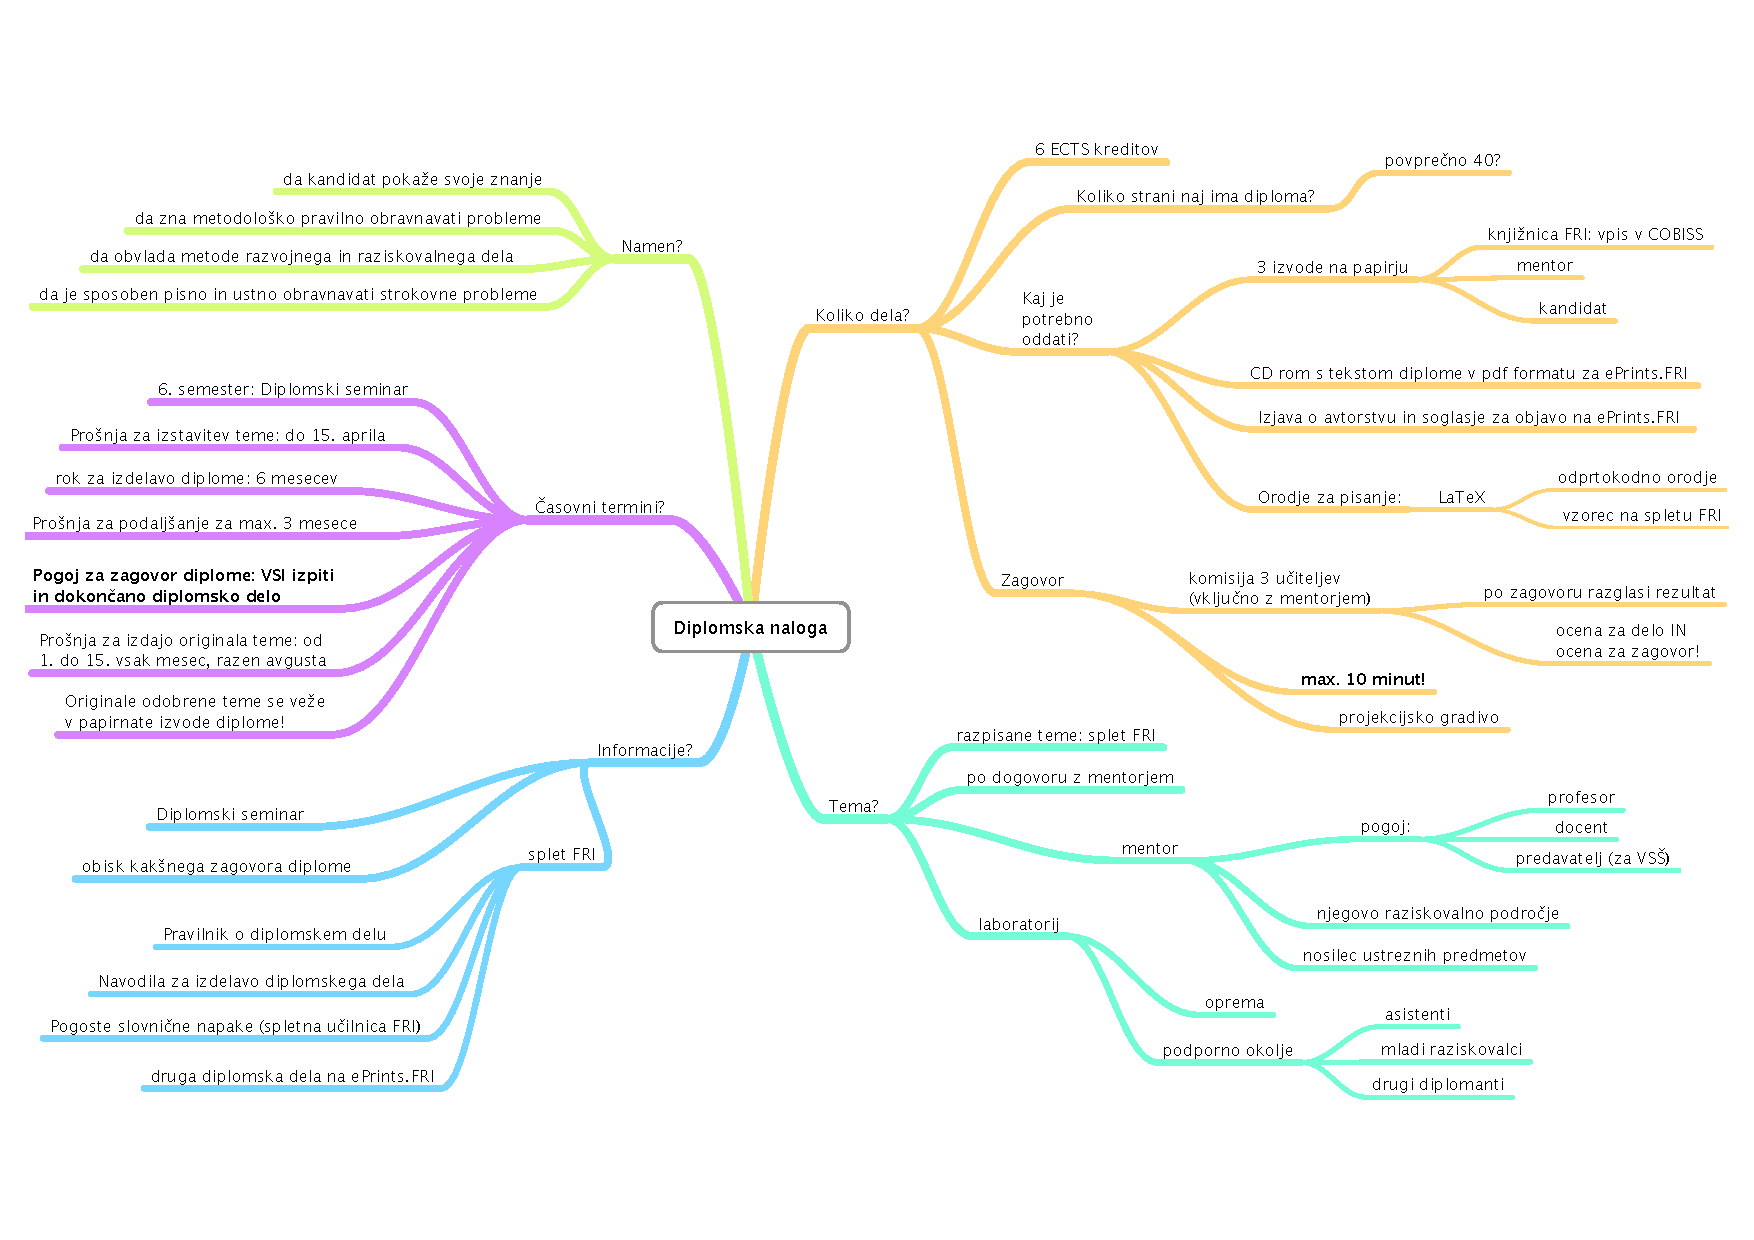
\includegraphics[height=1.0\textwidth, angle=90]{mindmap.pdf}}
\caption{Miselni vzorec za mojo diplomsko nalogo.}
\label{sl:mindmap}
\end{figure}

Na posebni strani vključi dopolnjen miselni vzorec (Slika \ref{sl:mindmap}).



\section{Predvideni prispevki diplomske naloge}

Kaj bo rezultat diplomskega naloge? 
Neka nova programska oprema, ki bo reševala določeno nalogo?
Demonstracija neke obstoječe rešitve in metode na novem problemskem področju? 
Kako boš uporabljene ali razvite rešitve v diplomi preveril?


\section{Uporabljena metodologija}

Katera orodja in razvojno okolje boš uporabil in zakaj? 
Katere metode nameravaš preizkusiti?
Kako boš pridobil testne podatke?


\section{Razdelitev potrebnega dela na aktivnosti}

Sestavi spisek aktivnosti in podaktivnosti, ki te bodo pripeljale do konca diplome. Uporabi okolje ``enumerate''.
Za vsako aktivnosti določi, katere aktivnosti morajo biti dokončane pred obravnavano aktivnostjo in  konkretno akcijo, ki bo začela reševati oziroma bo pokrenila aktivnost.

Oceni trajanja vsake aktivnosti in posledično trajanje celotne izdelave diplomskega dela. Katere so kritične aktivnosti?


\section{Preliminarno kazalo}

Sestavi preliminarno kazalo diplomske naloge. Razdelitev na poglavja in podpoglavja naredi v okolju ``enumerate'' in pri vsakem v enem ali dveh stavkih zapiši o čem bo poglavje govorilo.

Celotna dispozicija naj bo dolga pet strani, vključno s slikami in seznamom literature.


\section{Seznam literature}

Za izdelavo seznama literature uporabi  Bib\TeX!


\bibliographystyle{plain}
\bibliography{literatura}

\end{document}  




